\documentclass[]{article}
\usepackage{amsmath}
\usepackage{amsthm}
\usepackage{listings}
\usepackage{graphicx}
\usepackage{hyperref}

\title{Practical Lab Numerical Computing Computational Finance \\Bachelor-Worksheet 4}
\author{Lukas Troska, Ilja Kalmykov}
\date{}
\setlength{\parindent}{0pt}

\begin{document}

\maketitle

The referenced source code files can be found on
\url{https://github.com/iljaGH/CompFin/}.

\section*{Task 1}
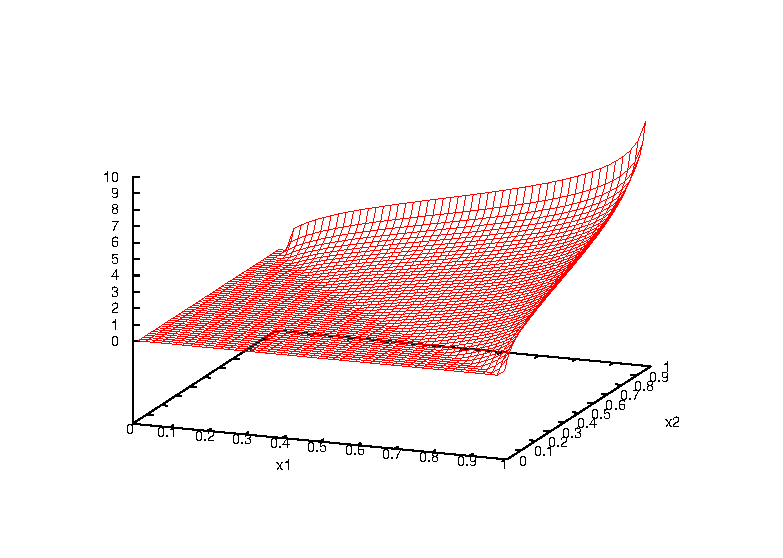
\includegraphics[width=.9\textwidth]{task1.eps}\\

\section*{Task 2}
Below are the two convergence plots for MC and QMC respectively. The third plot is a pseudo-convergence plot of MC using a low precision reference value. We see that the plot stabilizes at a higher "error".

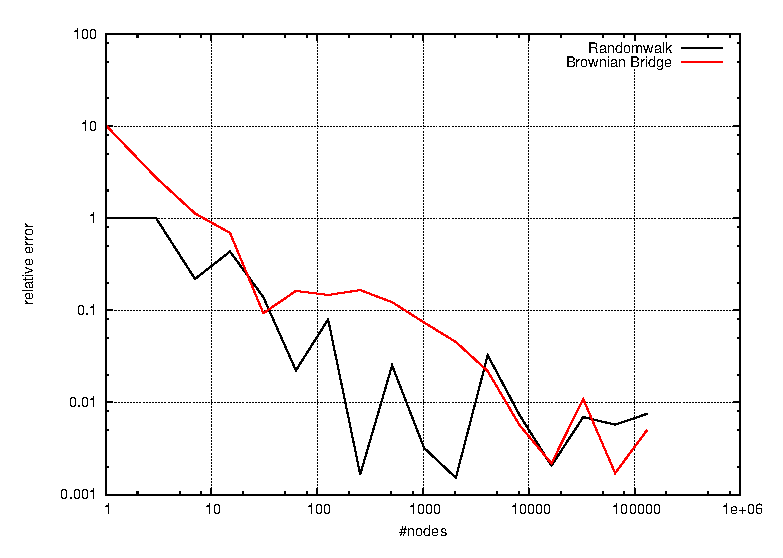
\includegraphics[width=.9\textwidth]{task2_mc_high.eps}\\
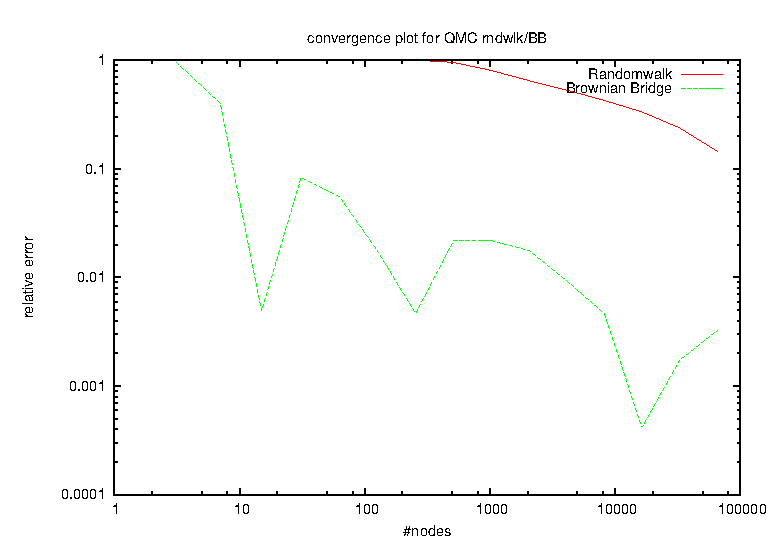
\includegraphics[width=.9\textwidth]{task2_qmc.eps}\\
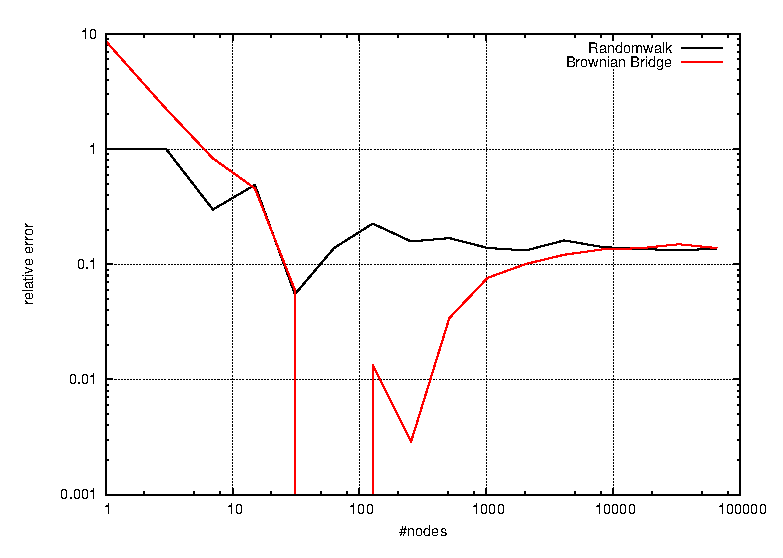
\includegraphics[width=.9\textwidth]{task2_mc_low.eps}\\

\section*{Task 3}
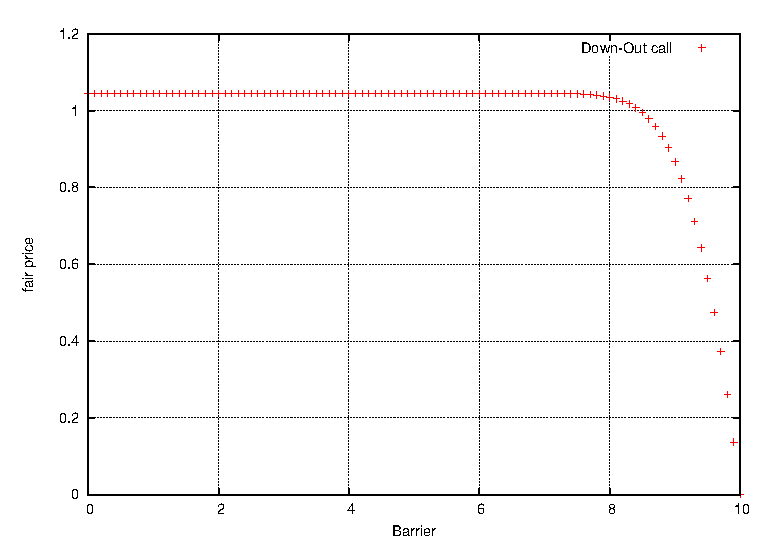
\includegraphics[width=.9\textwidth]{task3.eps}\\

\section*{Task 4}
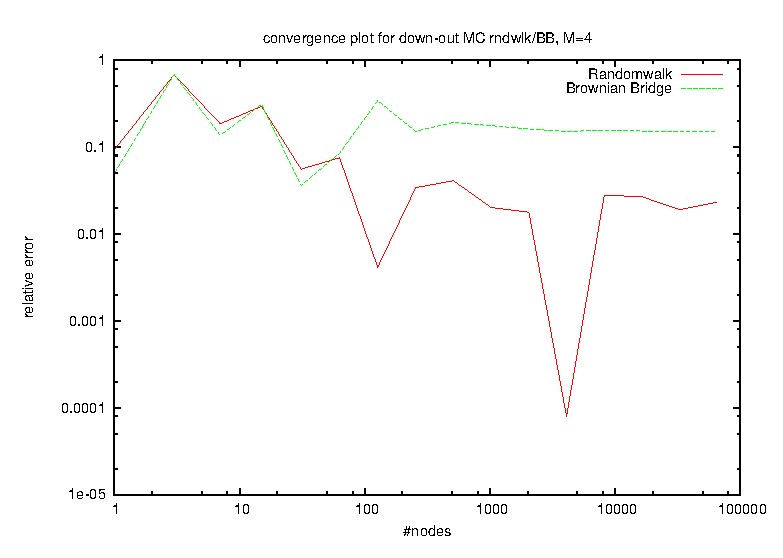
\includegraphics[width=.9\textwidth]{task4_mc_4.eps}\\
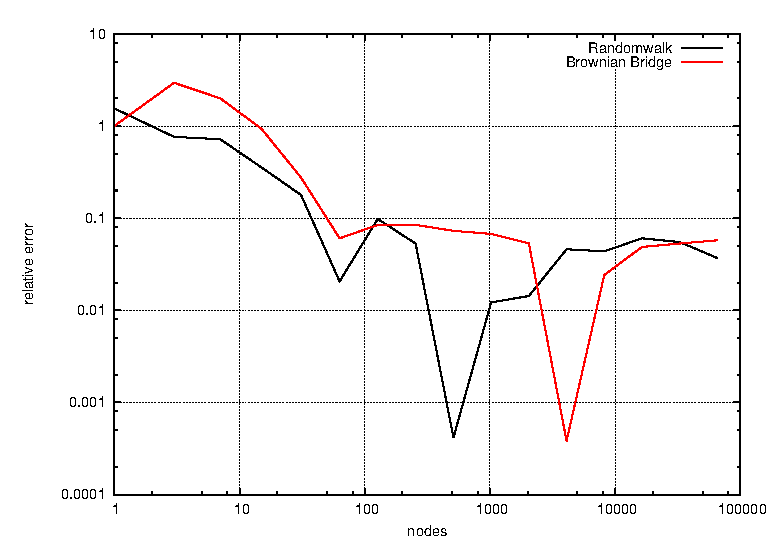
\includegraphics[width=.9\textwidth]{task4_mc_64.eps}\\
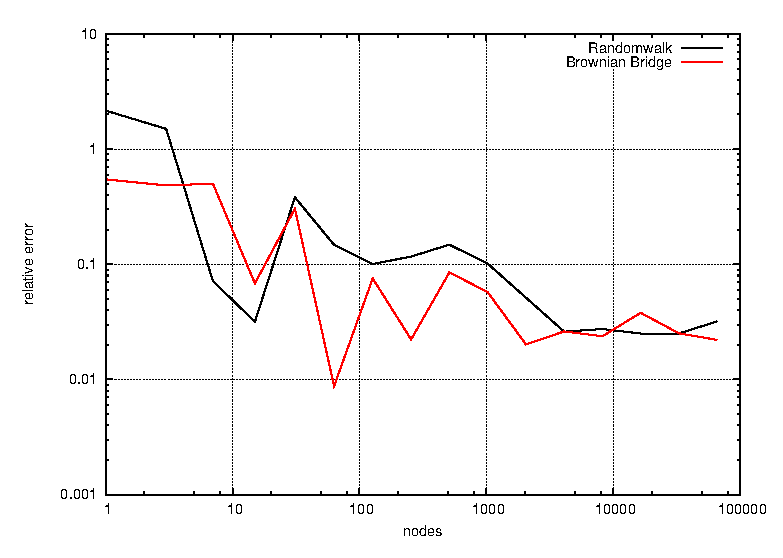
\includegraphics[width=.9\textwidth]{task4_mc_256.eps}\\
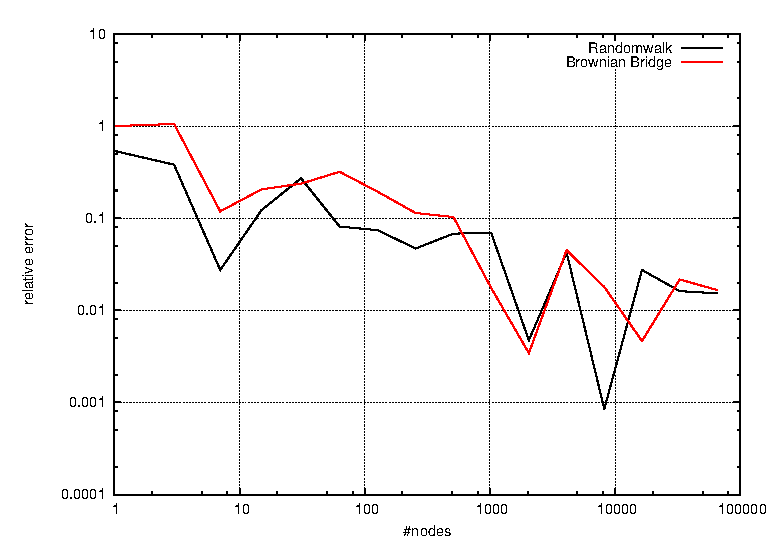
\includegraphics[width=.9\textwidth]{task4_mc_1024.eps}\\

\section*{Task 5}
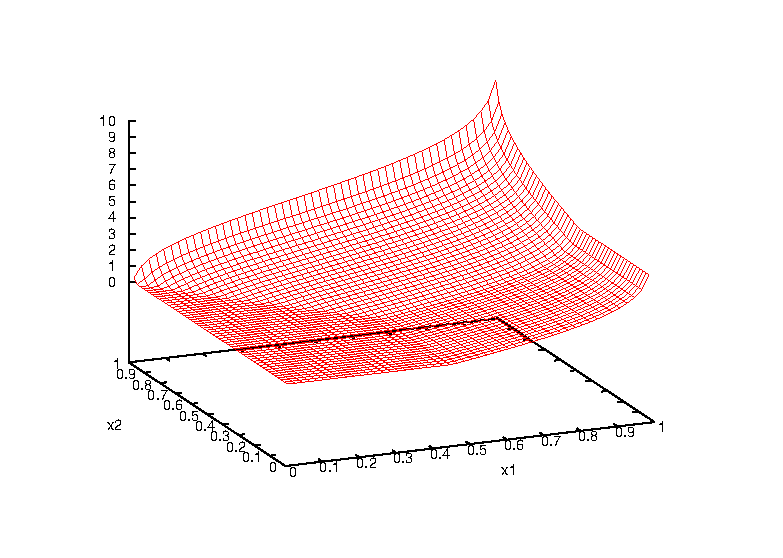
\includegraphics[width=.9\textwidth]{task5.eps}\\

\section*{Task 6}
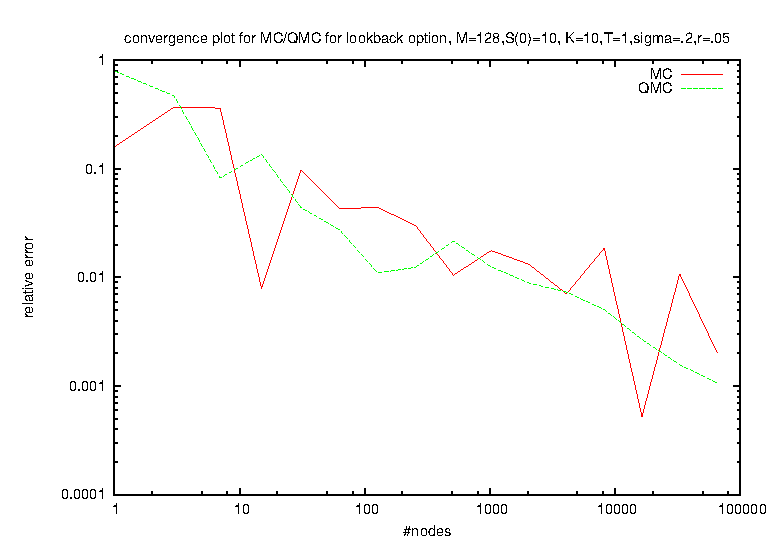
\includegraphics[width=.9\textwidth]{task6.eps}\\

\section*{Task 7}
See task7.cpp for code.

\section*{Task 8}
See task8.cpp for code.

\section*{Task 9}
The following is a plot of the implied volatility of a Lufthansa call option, with $T=0.1$. At the time, Lufthansa stock was worth $19.93$, and the options were valued:\\
$\begin{array}{c|c}
K & V\\
\hline
19.5&0.97\\
19.75&0.79\\
20&0.65€\\
20.25&0.54€\\
20.5&0.44€\\
20.75&0.36€\\
21&0.3€\\
\end{array}$\\
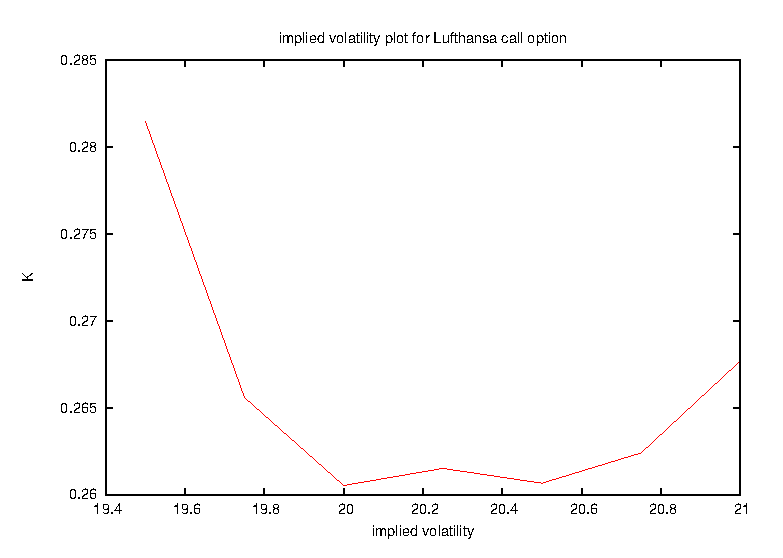
\includegraphics[width=.9\textwidth]{task9.eps}\\
\end{document}
